% Created 2019-07-24 Wed 15:01
% Intended LaTeX compiler: pdflatex
\documentclass[letterpaper, 11pt]{article}
\usepackage[utf8]{inputenc}
\usepackage[T1]{fontenc}
\usepackage{graphicx}
\usepackage{grffile}
\usepackage{longtable}
\usepackage{wrapfig}
\usepackage{rotating}
\usepackage[normalem]{ulem}
\usepackage{amsmath}
\usepackage{textcomp}
\usepackage{amssymb}
\usepackage{capt-of}
\usepackage{hyperref}
\usepackage{natbib,graphicx,tikz,float,ragged2e,amsmath,amssymb,tabularx,subfig}
\usepackage[margin=1in]{geometry}
\renewcommand{\baselinestretch}{1.5}
\author{Amira Al-Khulaidy and Valentin Vergara}
\date{\today}
\title{Corruption and the effects of influence within social networks: An agent-based model of the “Lava Jato” scandal.}
\hypersetup{
 pdfauthor={Amira Al-Khulaidy and Valentin Vergara},
 pdftitle={Corruption and the effects of influence within social networks: An agent-based model of the “Lava Jato” scandal.},
 pdfkeywords={},
 pdfsubject={},
 pdfcreator={Emacs 26.2 (Org mode 9.1.9)}, 
 pdflang={English}}
\begin{document}

\maketitle
\begin{abstract}
Corruption, and more specifically corruption in Latin America, is a complex phenomenon which is affected by politics, social structures and institutions, as well as individual behaviors. The \textit{Lava Jato} is a large-scale example of corruption in Brazil. As of early 2019, there is still an ongoing investigation surrounding what has been lauded as the largest corruption scheme in Latin America. Advances in data analysis, computation, and social networks have allowed progress to be made with these types of investigations. The \textit{Lava Jato} case has been a clear example of how breaking up social networks and understanding the extent of crime and individual corruption has revealed webs of corruption that have influenced politics, as well as hindered economic developed in Brazil. The several layers of interactions between individuals and institutions can be difficult to grasp and understanding the patterns and relationships within complex large-scale phenomena, such as corruption can seem impossible. Agent-based models can help with understanding these complex behaviors and systems. By capturing the patterns and gaining a better understanding of how corruption emerges and is manifested, we can help inform policy, as well as create better tools and methods for crime prevention and detection. 
\end{abstract}

\section{Introduction}
\label{sec:orgac54265}

Corruption in Latin America has been a topic of interest across many fields. The historical, social and political roots of Latin America are deeply tied to the origins of the socio-political systems that govern many Latin American countries \citep{weyland1998}. Latin America has been at the forefront of political and economic discussions for decades, however, more recently, several webs of events have emerged, and the effects are long reaching with more complex ramifications. Corruption tends to focus on financial and political power, but in Latin America, there are several  aspects that make the topic of corruption more complex in terms of the financial and legal intricacies \citep{goldstein2018}. This paper is focused specifically on corruption in Latin America, and more specifically on the \emph{Lava Jato} corruption scheme and in Brazil. 

The reach and intermingled web of  the \emph{Lava Jato} scheme has had global implications, with many contributing factors. The complex interactions of individuals, institutions, and transactions can be better explored in an agent-based model (ABM) with a focus on the social networks of the agents. ABMs and social network analysis (SNA) allow us to capture the patterns from data to build a model, and then run the simulation to understand the patterns and results of the phenomenon we are investigating. From the model we can better capture what are the more prominent patterns, to gain a better understanding of how the different processes interact \citep{gilbert2005}.

By building a social network and running the model through time, we can derive a better understanding of how the \emph{Lava Jato} corruption scheme occurs, and how the impact of the various factors give rise to corrupt agents within a network. To better understand these factors, we will look at the different players and how their relationships enable this level of corruption based on whether agents engage in corruption, as well as their risk aversion which represents whether or not they engage in criminal behavior. We aim to look at how the social networks are formed and if different social networks have different outcomes in terms of the frequency of corrupt behavior. 

The importance of understanding corruption in a dynamic way is that law enforcement entities can experiment with different ways of targeting corruption. Ultimately, models and experiments that can be done for corruption detection, as well as understanding patterns for prevention can help with the social inequities that arise from misdistribution of funds and abuses of power.

\section{Background}
\label{sec:org78256a0}

\emph{Operacao Lava Jato}, or "operation car wash" is an ongoing investigation by the Federal Police of Brazil in the Southern part of Brazil \citep{federal_2018}. Beginning in 2014 and currently (2019) still ongoing, the scale of corruption has ranged from elected officials, to private companies, as well as cartels and off-shore banks- which has provoked public uproar, protests and political upheavals in Brazil \citep{goldstein2018}. The initial investigation, which gave origin to the title of the operation was set to focus on \emph{doleiros}, black market money dealers, who used petrol stations and car washes to launder the profits of crime. The interactions of individual agents with criminal activity from the “bottom-up” gave rise to the emergence of one of the largest, if not largest corruption scandal in Latin America, if not the world \citep{angelico2017}. 

Several other investigations related to “Lava Jato” came to the forefront, including the beef and poultry industries. Sanctions were placed by other countries on imports from Brazil, which led to a cycle of effect that impacted consumer options and choices in homes around the world, which in return has resulted in an impact on the Brazilian Stock Market \citep{correa2018}. Sergio Moro, the federal judge responsible for the persecutions states that these types of crimes “represent a challenge for law-enforcement agencies” and that the level sophistication and the lack of tools and resources to deal with these types of crimes have allowed for years of corruption to go undetected and unpunished \citep{moro2018}.

While the investigation has yielded trials and arrests, there has been controversy surrounding the methods used for investigation and non-traditional means of persecuting these crimes \citep{lopes2016}. Previous scandals have also come to light, such as the \emph{Mensalao} (also known as Case 470) in 2002, but the results of previous investigations have not resulted in the scale and outcomes of the \emph{Lava Jato} investigation. The reason has been a delay in the justice system which make it harder for people of power to be tried \citep{moro2018}.  The defendants from this case have been politicians, CEOs, judges, cartels, and large corporations. Politicians who engage in corruption through their individual actions do impact policy, and political outcomes- “corruption can change the alignment of citizen and leader preference” \citep{besley2006}.

Corruption in Brazil has its origins in the history and political narrative of the country \citep{lopes2016}. More recently, the \emph{Mensalao} or Case 470 had been a controversial investigation where the vulnerabilities of the Brazilian legal system had come to the forefront. Due to the slow and bureaucratic nature of the legal system, \emph{Foro Privilegiado} required all political figures and elected public servants to be trailed exclusively by the Supreme Court \citep{moro2018}. This delayed the trails by a decade, which in addition to the corruption and political clout that exempted many from actually being trialed, corruption continued on with impunity. With the \emph{Lava Jato}, there have been changes to the justice system, focusing on speedier trails, repatriation, as well as quicker arrests of those involved in corruption and crimes. The openness and publicity involved in these entails, as well as the open resources online for denouncing crime have allowed us to have more data in terms of who the corrupt people are, as well as their network and how all the people connect to one another \citep{angelico2017}. 

As we gain a better understanding of the linkages between the major players in the \emph{Lava Jato} case, we can better understand the patterns of corruption in this case, and how individual choices from the bottom-up have created large scale corruption by looking at individual choices with an understanding of human psychology and sociology \citep{besley2006}. Why and how people choose to commit or not commit crimes and engage in corruption is a complex issue, but many psychologists \citep{milgram1963,raven1958} have looked at group behavior and power dynamics to better understand how people act and react within a social context, as well as tipping points of when people decide to adopt a behavior or not \citep{centola2005}. The “infectious” nature of how behaviors are adopted in social settings is the aim of this paper, and we hope to expand some of these thoughts to examine the corruption of individuals involved in the \emph{Lava Jato} scheme through modeling this behavior.

Specifically, an agent-based model can help understand the patterns of these relationships, and theories or how power and influence can have a larger effect on individual choices. The more powerful an individual, the more power it holds in a social web. In the specific case of \emph{Lava Jato}, we have the different agents, and their relationship to other agents. We also know which agents are more connected given the arrests from the investigation and the data from our proceedings \citep{garay18}.

The reach of corruption has been extensive, and the effects on political parties and campaigns have also tainted Brazilian politics and the trust of the people in the government. It would be impossible to reflect all of these different aspects in a model, but the focus of this paper is to understand the patterns of the social network and the \emph{influence} \citep{centola2005} of people on their peers, and whether they are more or less likely to commit crimes. Categories used  includes the public sector, which includes public employees of any government institution; private sectors, referring to those people who carry out licit commercial activities outside the public sphere; full-time criminals, which covers those nodes/agents who regularly carry out activities defined as criminal offenses; and financial institutions and which groups agents/nodes belong to the financial system. These classifications allow us to better understand the organizational and institutional role of each agent, in addition to the particular characteristics of the structure of the network \citep{garay18}.

\section{A model for corruption}
\label{sec:orgeda23d5}

\subsection{General description}
\label{sec:org657365d}
The model we developed tries to recreate how corrupt behavior spreads in a network structure, and how the cumulative effects of corruption cases discovered by the public
opinion behave in a reasonable period of time. We based some our assumptions and most of the model from the recent corruption cases in Brazil \citep{garay18}.

Past models have looked at corruption within government with an analysis of corruption and the effects on the effectiveness of Rule of Law \citep{guerrero2019}. Others have examined the micro and macro-level interactions of corruption with agent-based models within a game theory context \citep{hammond2000}. Our model hopes to look at the spread of corruption, specifically through a lens of influence of corruption on the agents within a network. We model the spreading of corruption in a network structure and describe with more detail the different networks that we will create and the processes underlying their changes. Then, we describe what our model does and the reasons behind our assumptions.

\subsection{Generation of networks}
\label{sec:orgb2ce29b}
For this model we used custom code, since we had to create networks where the nodes are the agents in our model. Examples of the networks chosen are in Figure \ref{fig:orgbe3c0a7}. The first network is a Random Network \citep{gilbert1959}. In an undirected network with \(n\) nodes, for every one of the possible \(\binom{n}{2}\) links, there is a probability \(p\) of creating that edge. The density of this network approaches \(p\). We then look at the \emph{Small World} network \citep{watts1998}. We started with a ring network where every node has degree 4\footnote{This means that every node is connected to the adjacent 2 in the "left" and in the "right", relative to its position in the ring.}. Then, for every link \((i, j)\) we broke it and created another link \((i, k)\) with probability \(p\), where \(k\) is a node chosen at random.

\begin{figure}[!h]
\centering
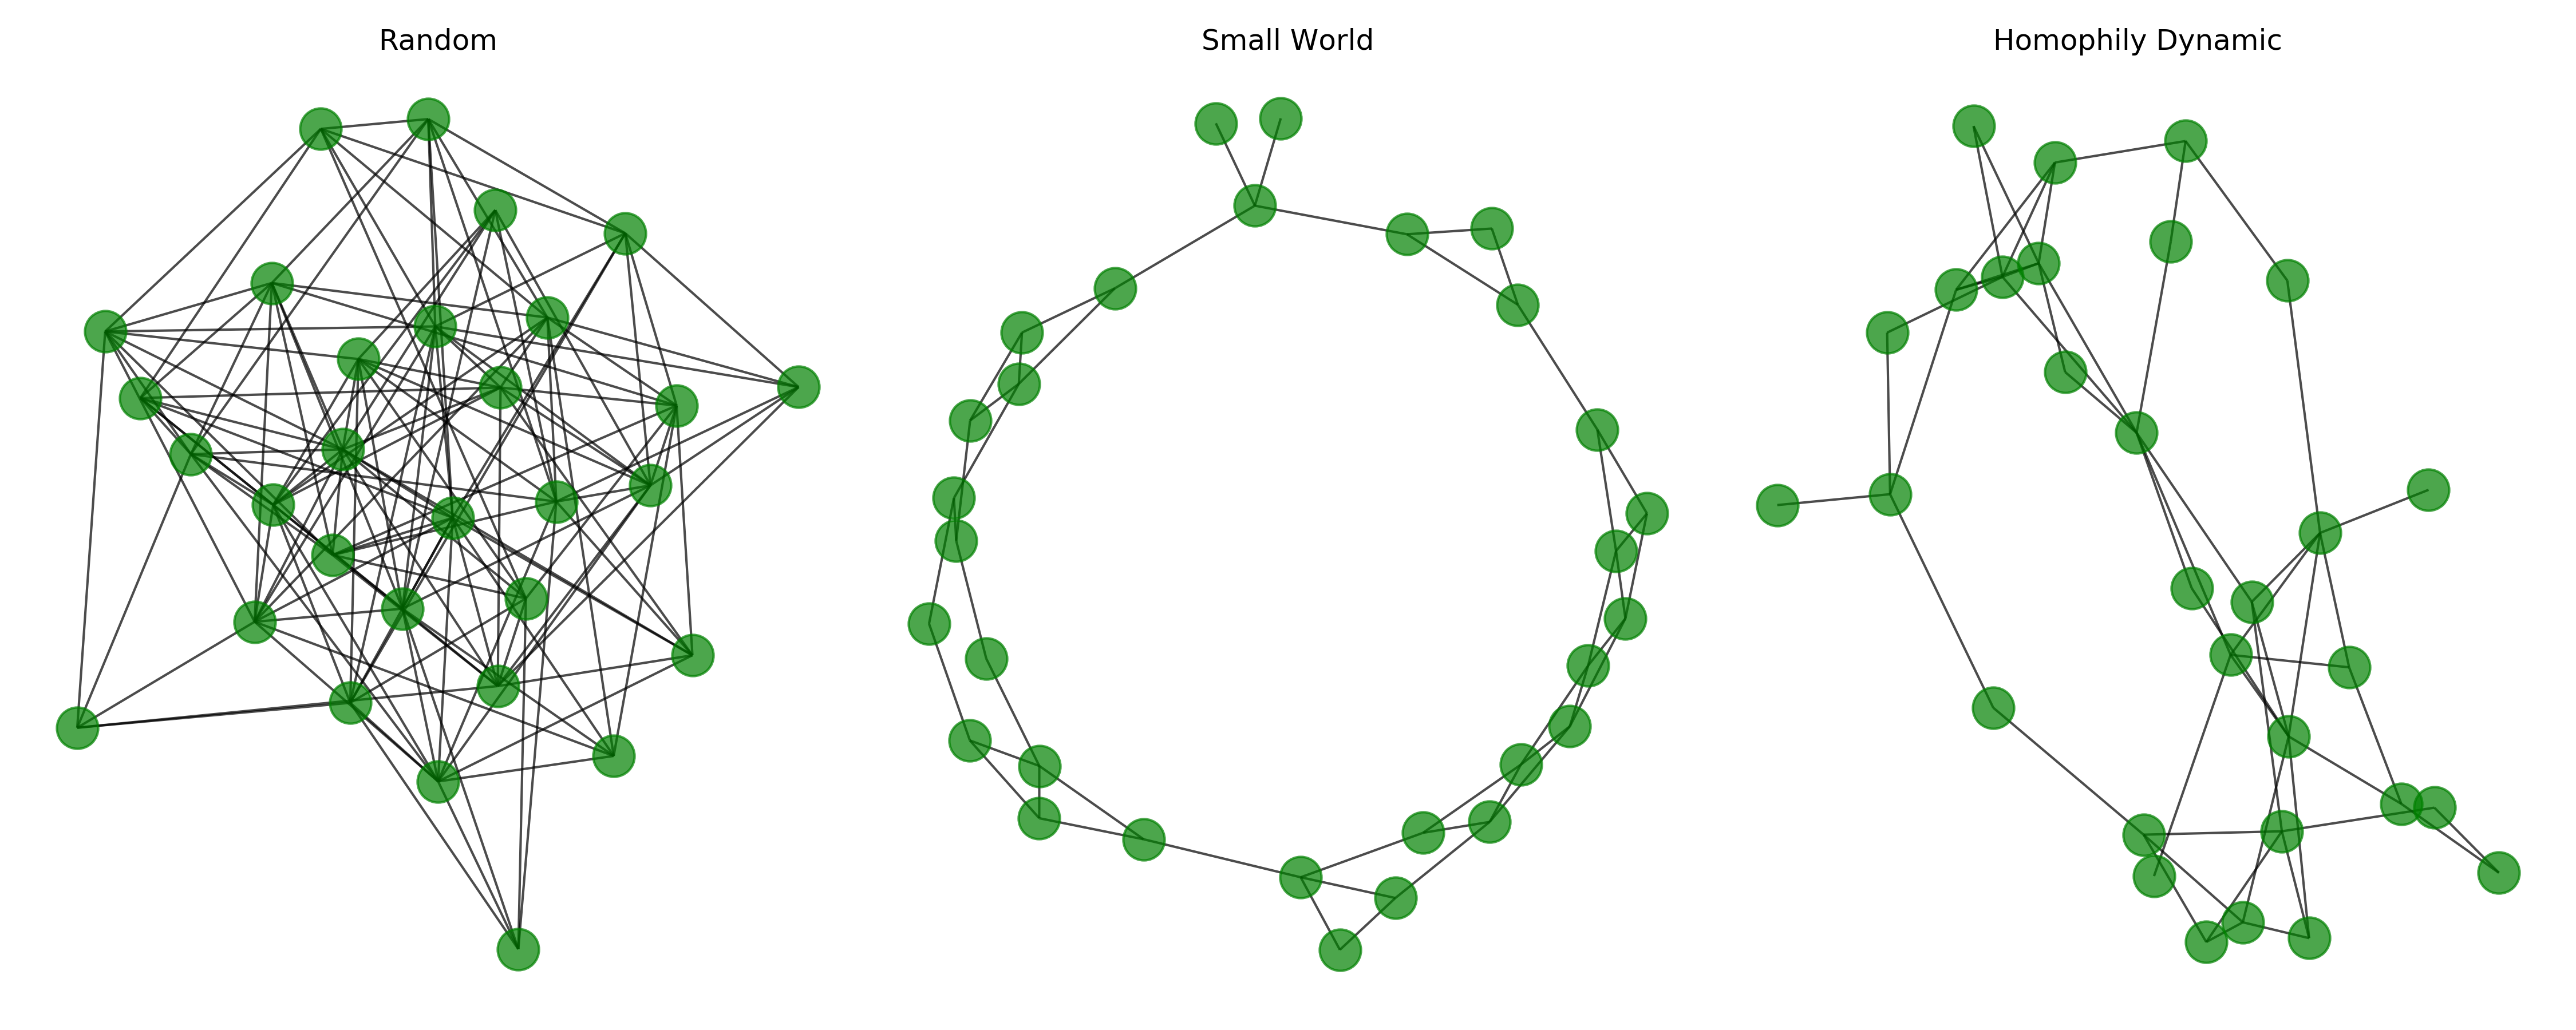
\includegraphics[width=.9\linewidth]{img/f1.png}
\caption{\label{fig:orgbe3c0a7}
Three network types used in our model.}
\end{figure}


The network on the right of Figure \ref{fig:orgbe3c0a7} is a Homophily Dynamic one, based on \citet{murase2019}. It is assumed that every node has some number of attributes \(f \in \{1, 2, \ldots, F\}\). Those attributes can take \(q\) different values, where \(2 \leq q \leq Q\). As \(F\) is increased, the social system becomes more complex, and as \(Q\) increases, the individuals become more heterogeneous. At every time step, the edges in the network may change based on the following three processes:

\begin{description}
\item[{Global Attachment (GA)}] A node selects one of its \(F\) attributes and chooses at random from the subset of nodes with the same \(q\) value in that attribute. They establish a link.
\item[{Local attachment (LA)}] A node \(i\) with \(k_{i} > 0\) chooses one of its neighbors, \(j\), who in turn, chooses one of its neighbors, \(k\) such that \(f_{j} = f_{k}\). Then, if \(i\) and \(k\) are not connected, a node is created.
\item[{Link deletion (LD)}] Every element in the edge set is removed with probability \(p_{d}\).
\end{description}

For the purpose of this research, we only used one attribute of the nodes as the \emph{homophily} variable : the political party of every node, choose at random at the initialization of the model with a uniform distribution between \(A\), \(B\), and \(C\).

\section{Attributes of the model}
\label{sec:org477d8d5}
Our model places the agents in a network, with the following attributes.

\subsection{Agents}
\label{sec:org03bb9d1}
In this artificial social system, agents can have one of three possible roles \citep{parsons1991}: they can belong to the private, public or criminal sector, which represents three of the major aspects of the \emph{Lava Jato} case. We chose the proportion of agents in each of the roles as 0.7, 0.19, and 0.11, respectively, as these proportions are based on empirical data from \citet{garay18}.

During the model, agents can be \textbf{corrupt} or not. This means that they engage in an illicit transaction where they get a payoff. We let the corrupt status of every agent be a random variable resulting on a Bernoulli trial with probability \(c\) of being corrupt.

Since every agent can be, at different parts of the model, in both ends of an illicit transaction, we created two attributes for this. The first one is a \textbf{transaction size} value, when the agents proposes the illegal exchange. This is the result of a random discrete variable with uniform distribution with domain \([100, 1000]\). What this variable represents is how big the transaction is, in terms of an abstract currency unit. The second attribute puts the agent at the other end and corresponds to the \textbf{risk aversion}, which is a random variable that draws from different distributions depending on the argument passed. The possible arguments are:

\begin{description}
\item[{\texttt{'u'}}] Uniform Risk Aversion. Uniform distribution between 0 and 1.
\item[{\texttt{'l'}}] Low risk aversion. \(\beta(2, 5)\) distribution. Biased to the left.
\item[{\texttt{'m'}}] Medium risk aversion. \(\beta(2, 2)\) distribution. Symmetrical centered around 0.5.
\item[{\texttt{'h'}}] High risk aversion. \(\beta(5, 2)\) distribution. Biased to the right.
\end{description}

Finally, agents keep track of their \textbf{political party} (random variable that chooses
between \(A\), \(B\), or \(C\), which were abstracted due to the many different political parties in Brazil); whether they are under \textbf{investigation} for corruption or not; and the total amount of payoff obtained from illegal transaction since the first time-step.

\subsection{Initialization of the model.}
\label{sec:org58dacc7}
When the model initializes, we create a \textbf{list} of the agents, with the proportions described above. After that, we take that list and make every item in it the node in a \textbf{network} using either a random, small world or homophily dynamic structure. At the beginning of every time step, we updated the network using a random rewiring or a homophily based one (with the GA, LA and LD processes in sequential order).

\subsection{Interactions}
\label{sec:orgb0b6b88}
Every time step is a week \(w\), which is chosen due to the nature of the transitions carried out and captures the frequency of the transactions based on all the interacting agents. Before any interactions, we choose a random number of transaction attempts \(\tau\). Then, for every one of those, we choose a random node i that will try to make an illegal transaction with node j. In case \(j\) is corrupt, the transaction happens and \(j\) gets as a payoff 5\% of the tranbsaction value (transaction size). In case \(j\) is not corrupt, it can accept the exchange with probability \((1 - \text{risk aversion})\). If the transaction is successful, \(j\) changes its status to corrupt and updates its payoff.

\subsection{Corruption punishment.}
\label{sec:org1a97377}
After all the transaction attempts have been made, the model checks the current value of the payoff for every agent. If it exceeds some value \(p^{*}\), the agent gets caught with a probability \(p_{c}\). When this happens, the caught agent goes to jail (is removed from the agent set and from the network) and all of its neighbors change their status to "under investigation" and increase their risk aversion. 

\subsection{New agents enter the model}
\label{sec:orgfd0cdde}
We replace every agent removed from the model, keeping the same proportion between criminal, public and private sectors. Since at the beginning of each \(w\) we will update the network, these "new agents" get connected with another node depending of the specific network structured used to do the update. 

\section{Model Experiments and Results}
\label{sec:orgb6a48ec}

\subsection{Baseline parameters}
\label{sec:org097db05}
To begin testing our abstract model, we established a set of parameters (in Table \ref{tab:org8a0c816}) with enough variability that will produce noticeable results, against which we will compare different variations.

\begin{table}[htbp]
\caption{\label{tab:org8a0c816}
Baseline parameters of the model}
\centering
\begin{tabular}{lr}
\hline
\hline
 & Initial values\\
\hline
Number of nodes & 500\\
Number of transaction attempts per week & \([20, 30]\)\\
Amount of payoff until agent gets investigated & 100\\
Probability of getting caught & 0.1\\
Proportion of corrupt agents & 0.2\\
Distribution of risk aversion & \texttt{'u'}\\
Network update process & GA, LA and LD\\
\hline
\hline
\end{tabular}
\end{table}

Based on these parameters, we created three networks, whose initial configuration was a random, small world and homophily network; and then let the model run for 52 weeks to capture the cycle of different transitions that occur within the private, public, and criminal sectors, and with an update process that uses GA, LA and LD \citep{murase2019} each week. At the end, the resulting networks are in Figure \ref{fig:org49f5a1f}. As expected, the random network looks like a hairball and depicts an unreal scenario where every node has random links. 

\begin{figure}[htbp]
\centering
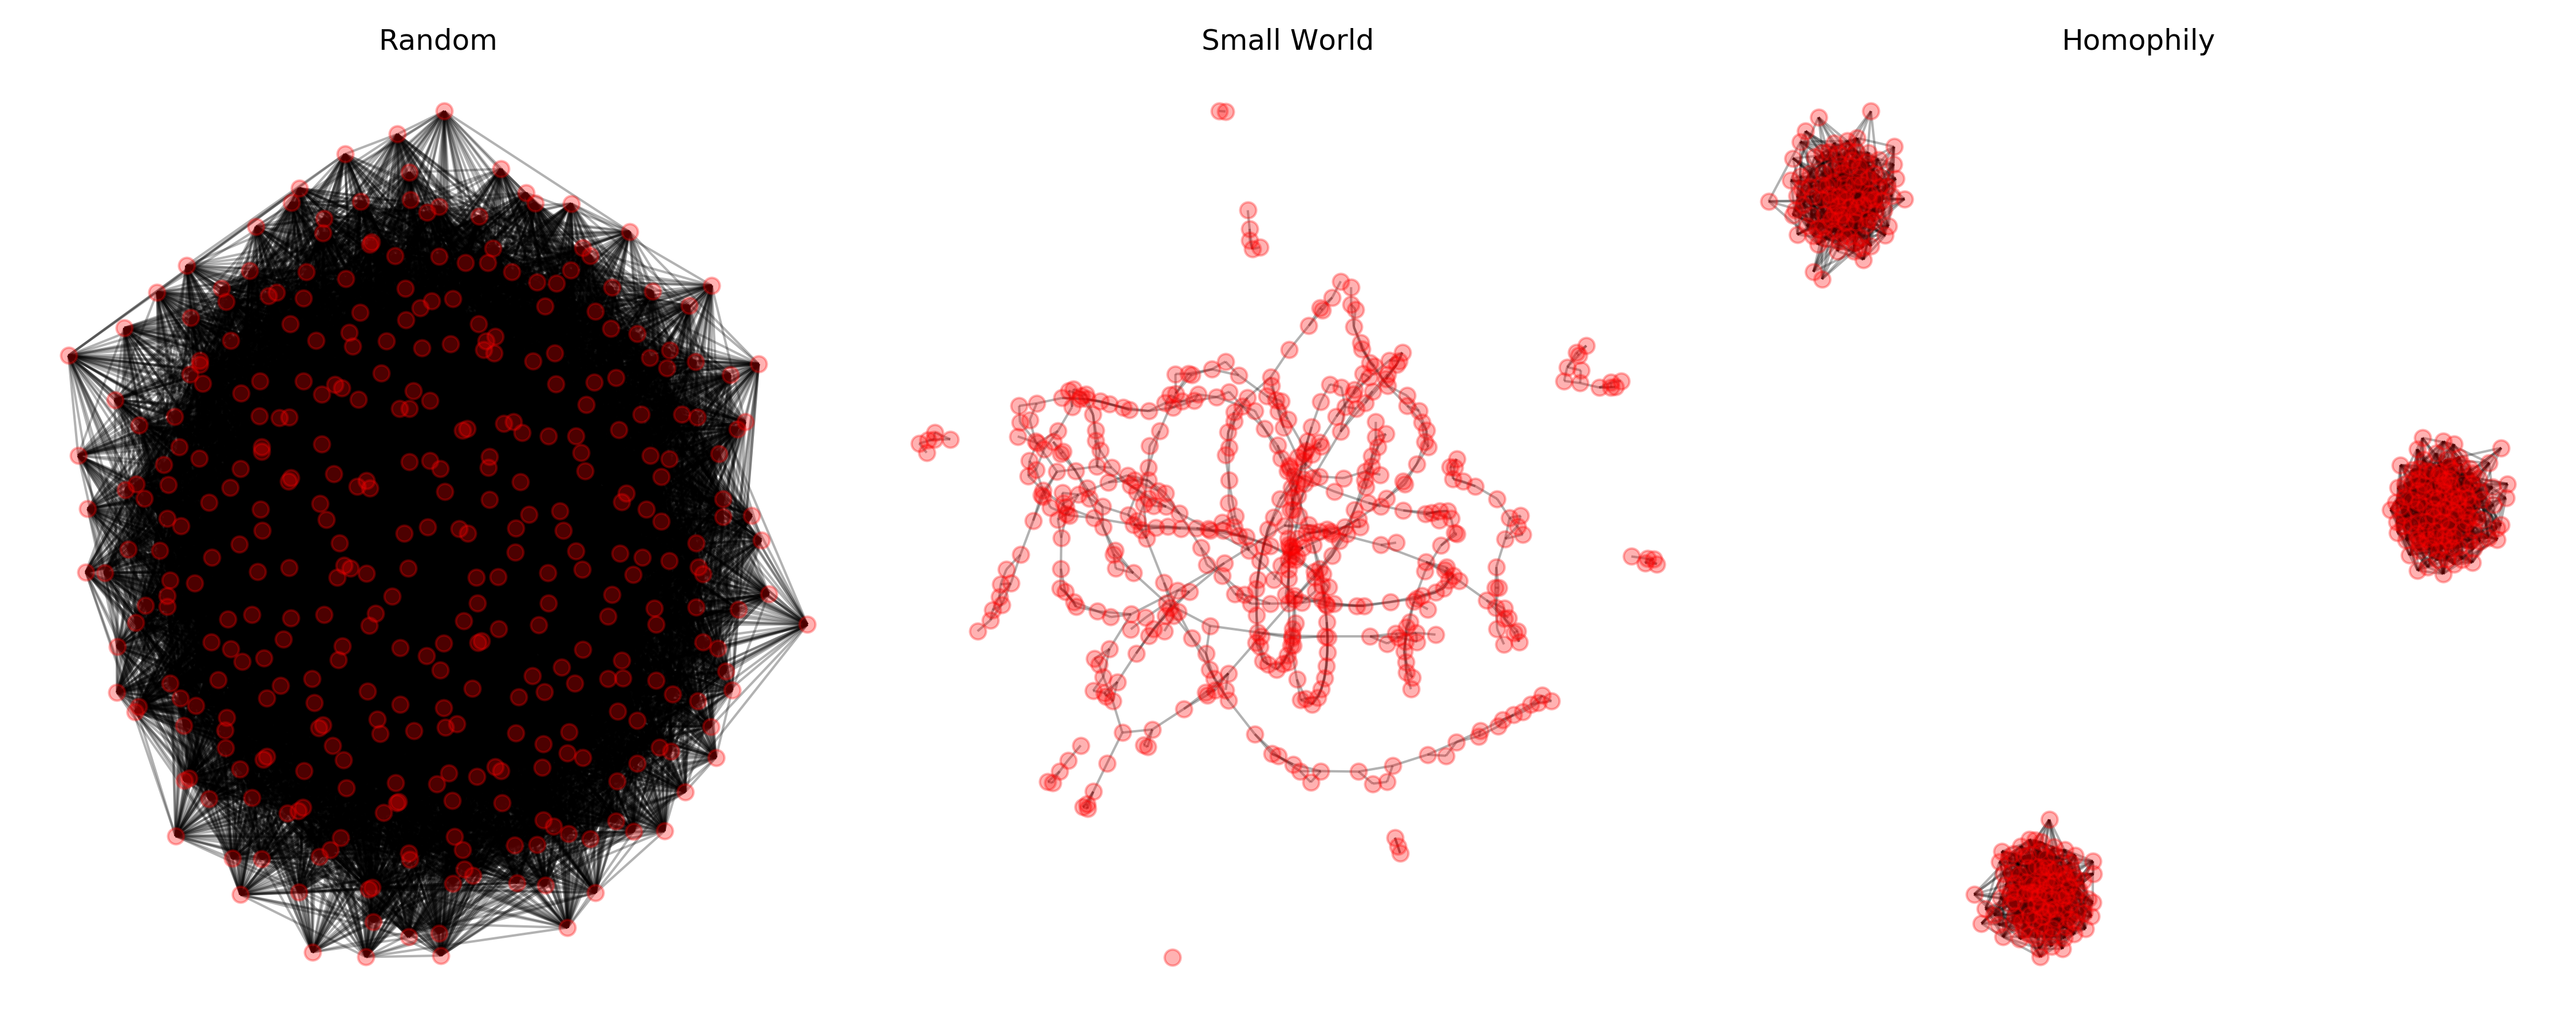
\includegraphics[width=.9\linewidth]{img/f2.png}
\caption{\label{fig:org49f5a1f}
Networks produced with baseline parameters at \(w=52\).}
\end{figure}

The network in the middle, the small world, has some characteristics that could be useful for the purposes of this research. For example, two nodes at random have a shortest path \(L\) that is proportional to \(\ln n\), where \(n\) is the number of nodes. In our example, this mean that from one node, it is easy to reach any other in the network. However, the fact that the nodes can easily reach the other does not mean that they can easily influence each other and spread corrupt behavior. That is the reason why we included the networks in the right, where every node will influence others through \emph{homophily}, defined here as the political party. The three distinct subgroups in the plot are the three political parties used in our model.

Besides the obvious differences in the shape of the three networks, they have different values in some of the usual measurements in networks. This differences can be closely inspected in Table \ref{tab:orgcc80923}. 

\begin{table}[htbp]
\caption{\label{tab:orgcc80923}
Differences in network measurements at \(w=52\), baseline parameters.}
\centering
\begin{tabular}{lrrr}
\hline
\hline
 & Random & Small World & Homophily\\
\hline
Number of nodes & 330 & 491 & 306\\
Number of links & 9525 & 741 & 2467\\
Average Degree & 57.7273 & 3.0183 & 16.1242\\
Average Clustering & 0.1741 & 0.3492 & 0.1644\\
Average Path Length & 1.8246 & 6.2859 & 1.9136\\
\hline
\hline
\end{tabular}
\end{table}

To understand what happens inside these networks, over the one-year period, there are a few things to notice. First, the number of illegal transactions is depicted in Figure \ref{fig:org7d8e959} (top), where clearly we can see that in the small world network it remains stable, which is explained due to the low average degree compared to the other two networks. Since the nodes have less neighbors in average, they can \emph{ask} to do an illegal transaction to less people at every time step. 

\begin{figure}[htbp]
\centering
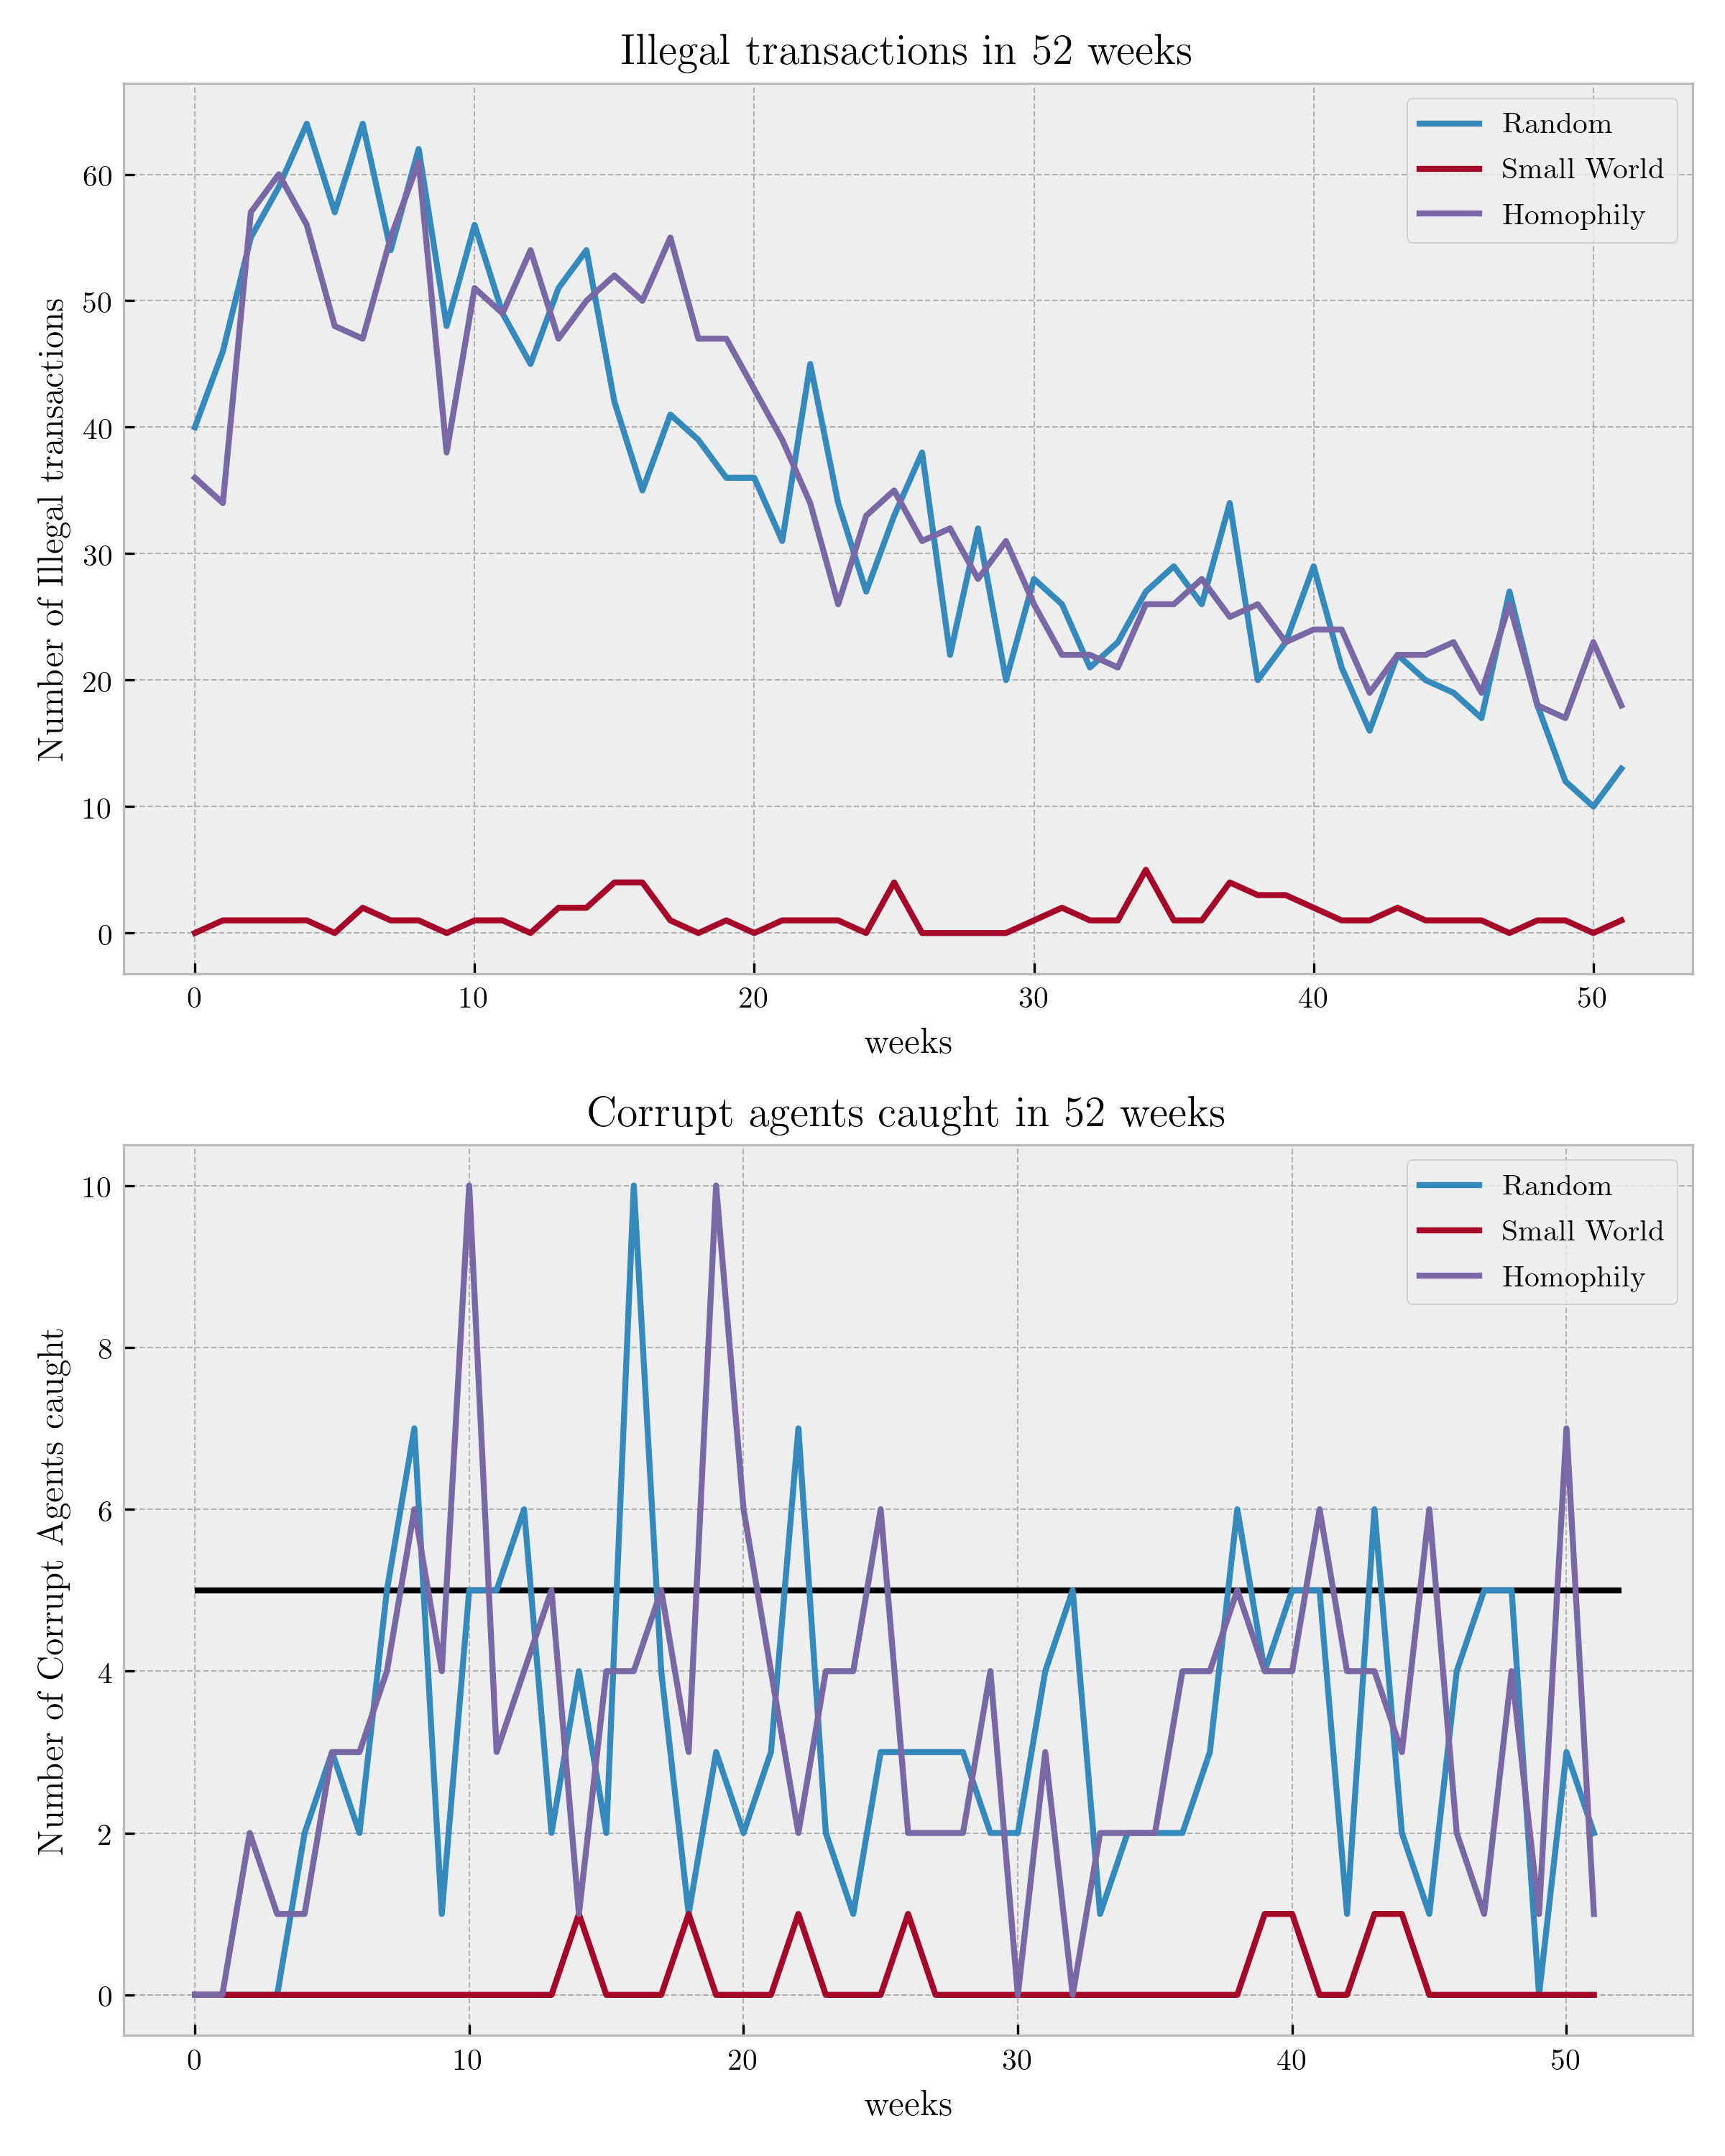
\includegraphics[width=.9\linewidth]{img/f3.png}
\caption{\label{fig:org7d8e959}
Number of illegal transactions, baseline parameters.}
\end{figure}

The second thing to look is the number of corrupt agents that get caught and are sent to jail. Figure \ref{fig:org7d8e959} (bottom) shows these results. We included a black horizontal line at 5 people caught. The reason is that in a given week, if more than 5 people get caught and are sent to jail for corruption, the whole social system will be on alert and could mean the beginning of what could resemble a corruption scandal. 

Both plots coincide in that the small world network has the fewest people involved in illegal transactions, and therefore, the fewest people caught. In the arbitrarily threshold we set, there is also evidence to support that homophily network will lead to more corruption scandals that the random network. In the homophily network nodes tend to influence other in their political party, and thus, when the corrupt agents are caught, it is easier to uncover the corruption acts of their neighbors.

\subsection{Modifying the network update mechanism.}
\label{sec:org57dace3}
In the baseline model, at every time step (every week) the network gets updated by a sequence of the GA, LA and LD processes. We tried running the three models in Figure \ref{fig:org7d8e959} by changing the network update process while all the other conditions remained the same. Instead of the sequence GA, LA, and LD, we updated the networks through a random process, where at every time step we broke all links and created new ones with probability \(p\).

The results in Figure \ref{fig:orgb1afed9}, as expected, show little difference between the three types of networks. All three are affected by the risk aversion increase at more or less the same rate, because every week new networks are created. 

\begin{figure}[htbp]
\centering
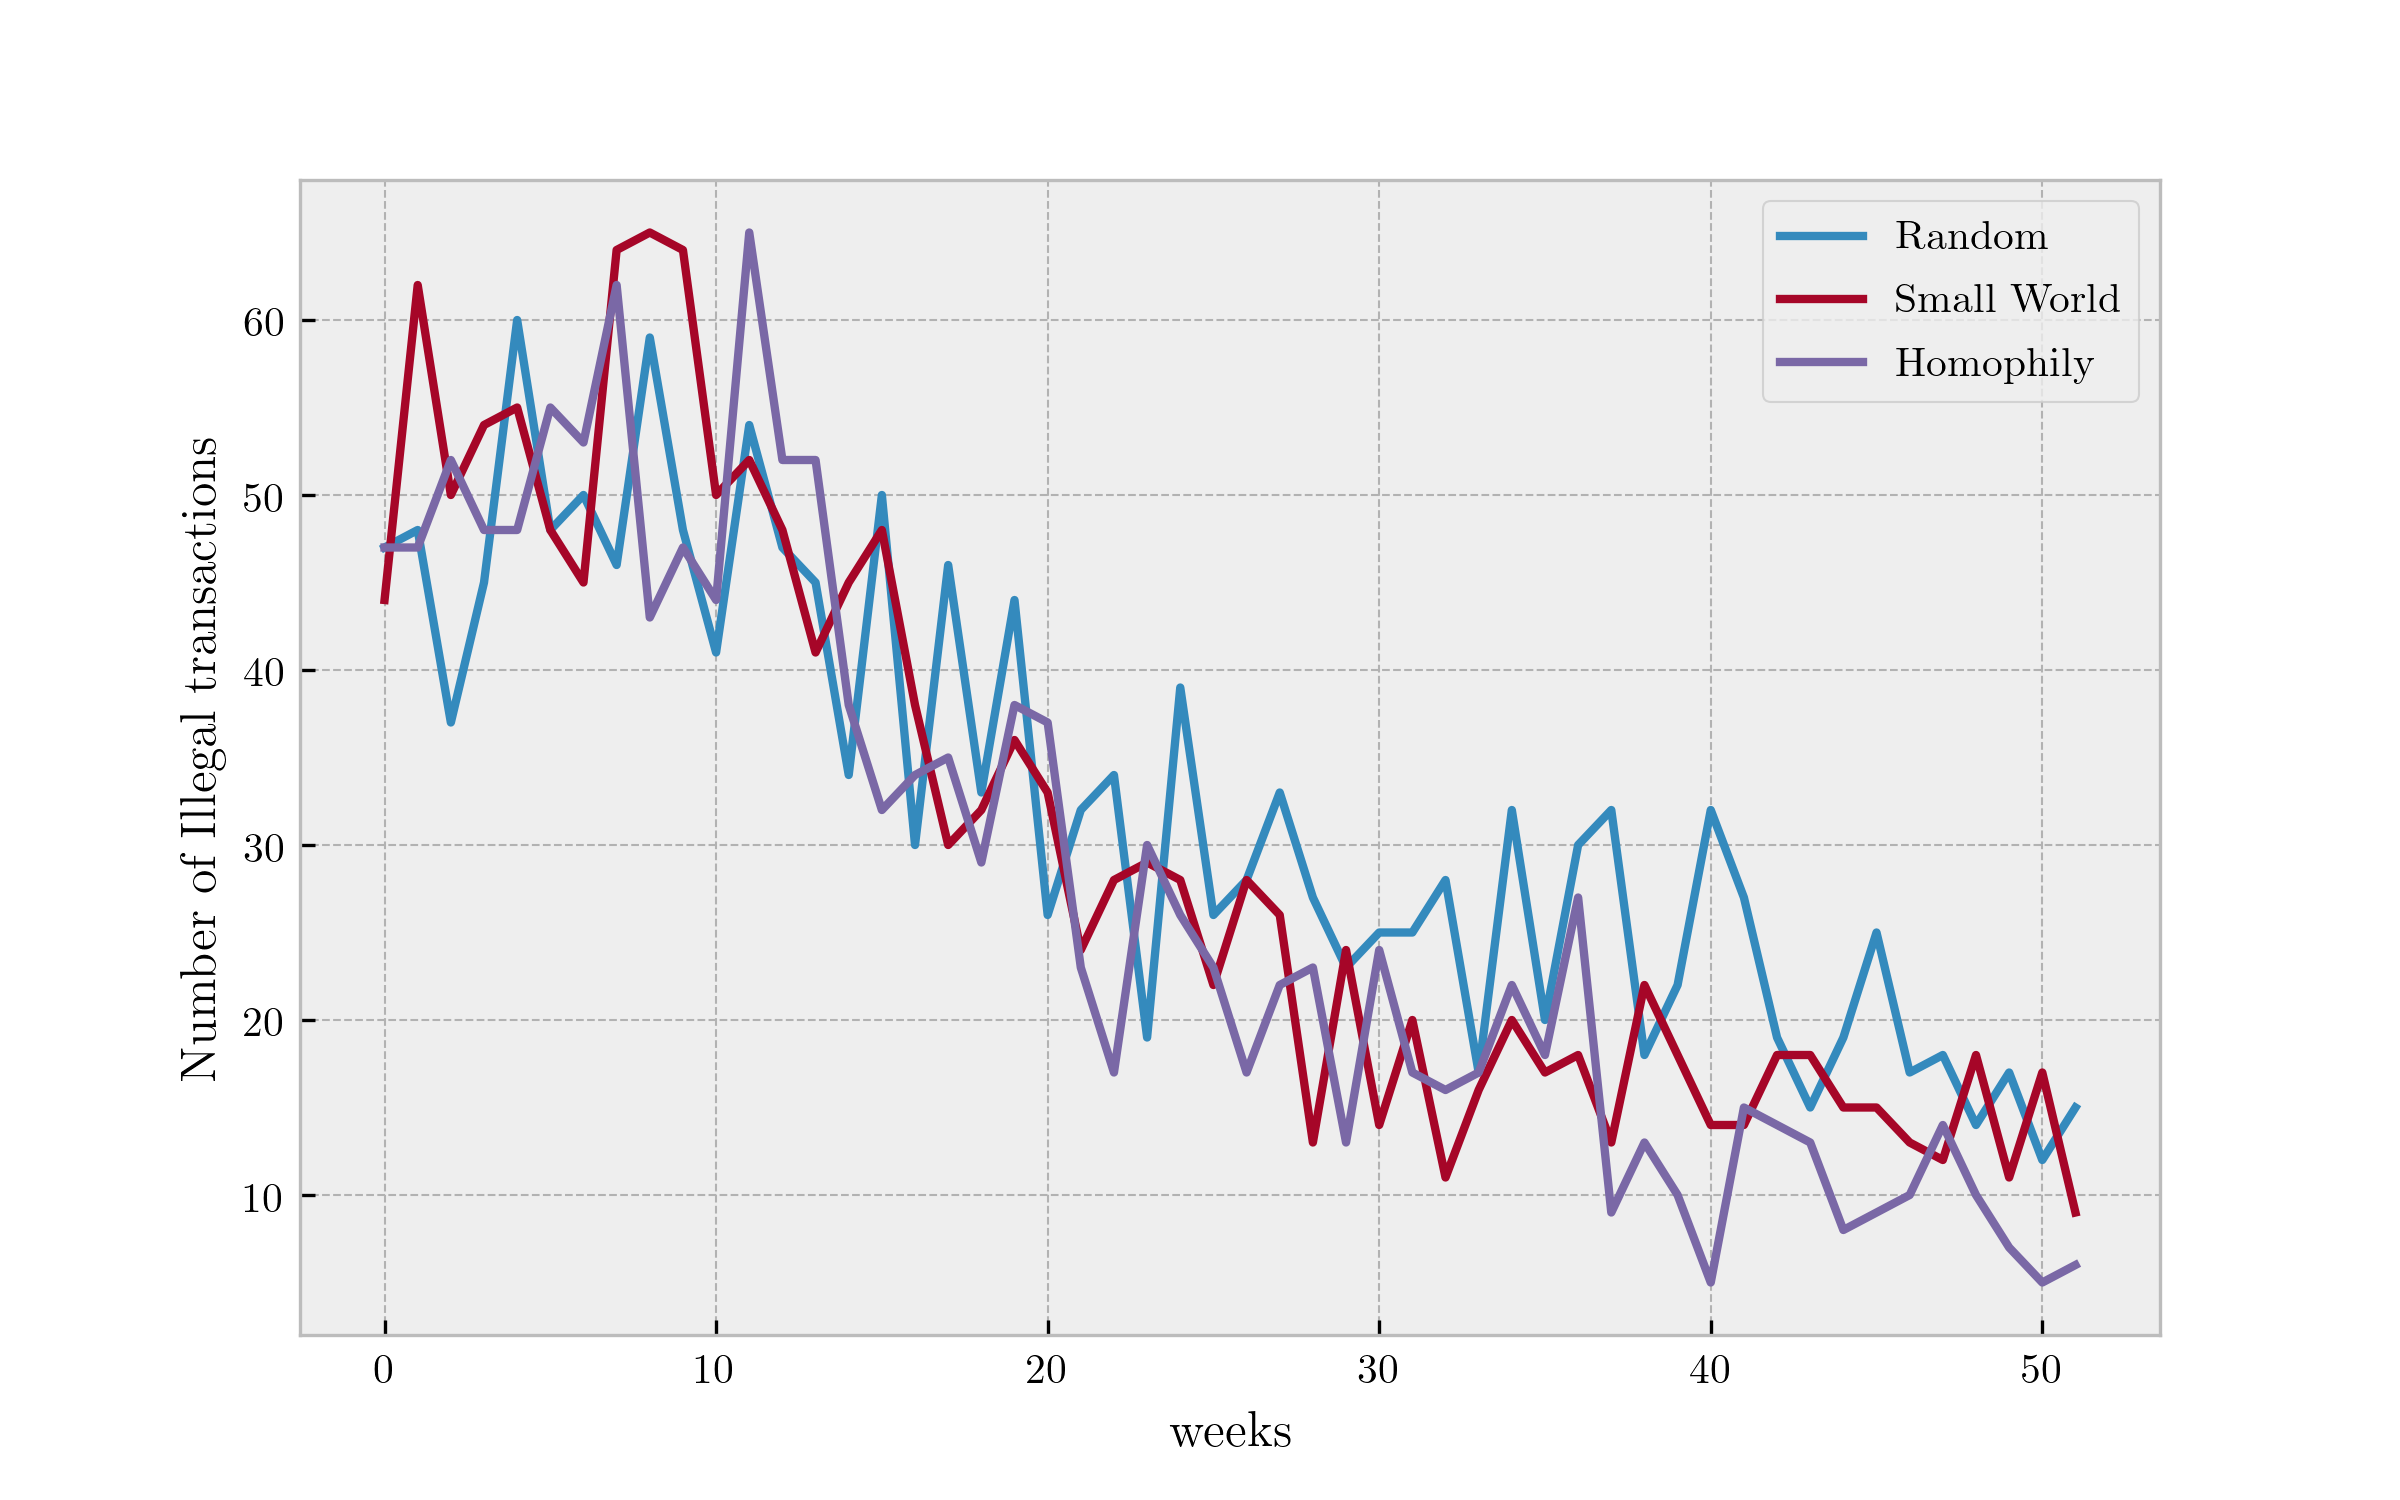
\includegraphics[width=.9\linewidth]{img/f4.png}
\caption{\label{fig:orgb1afed9}
Number of illegal transactions, with a random updating scheme.}
\end{figure}

\subsection{Effects of risk aversion}
\label{sec:org08fe74e}
Looking at our results so far, we decided to focus only on the homophily networks, since they capture more closely how people create political contacts. This is the reason why
Figure \ref{fig:org168b7a5} shows the effects of different distributions of risk aversion only for this type of network.

\begin{figure}[htbp]
\centering
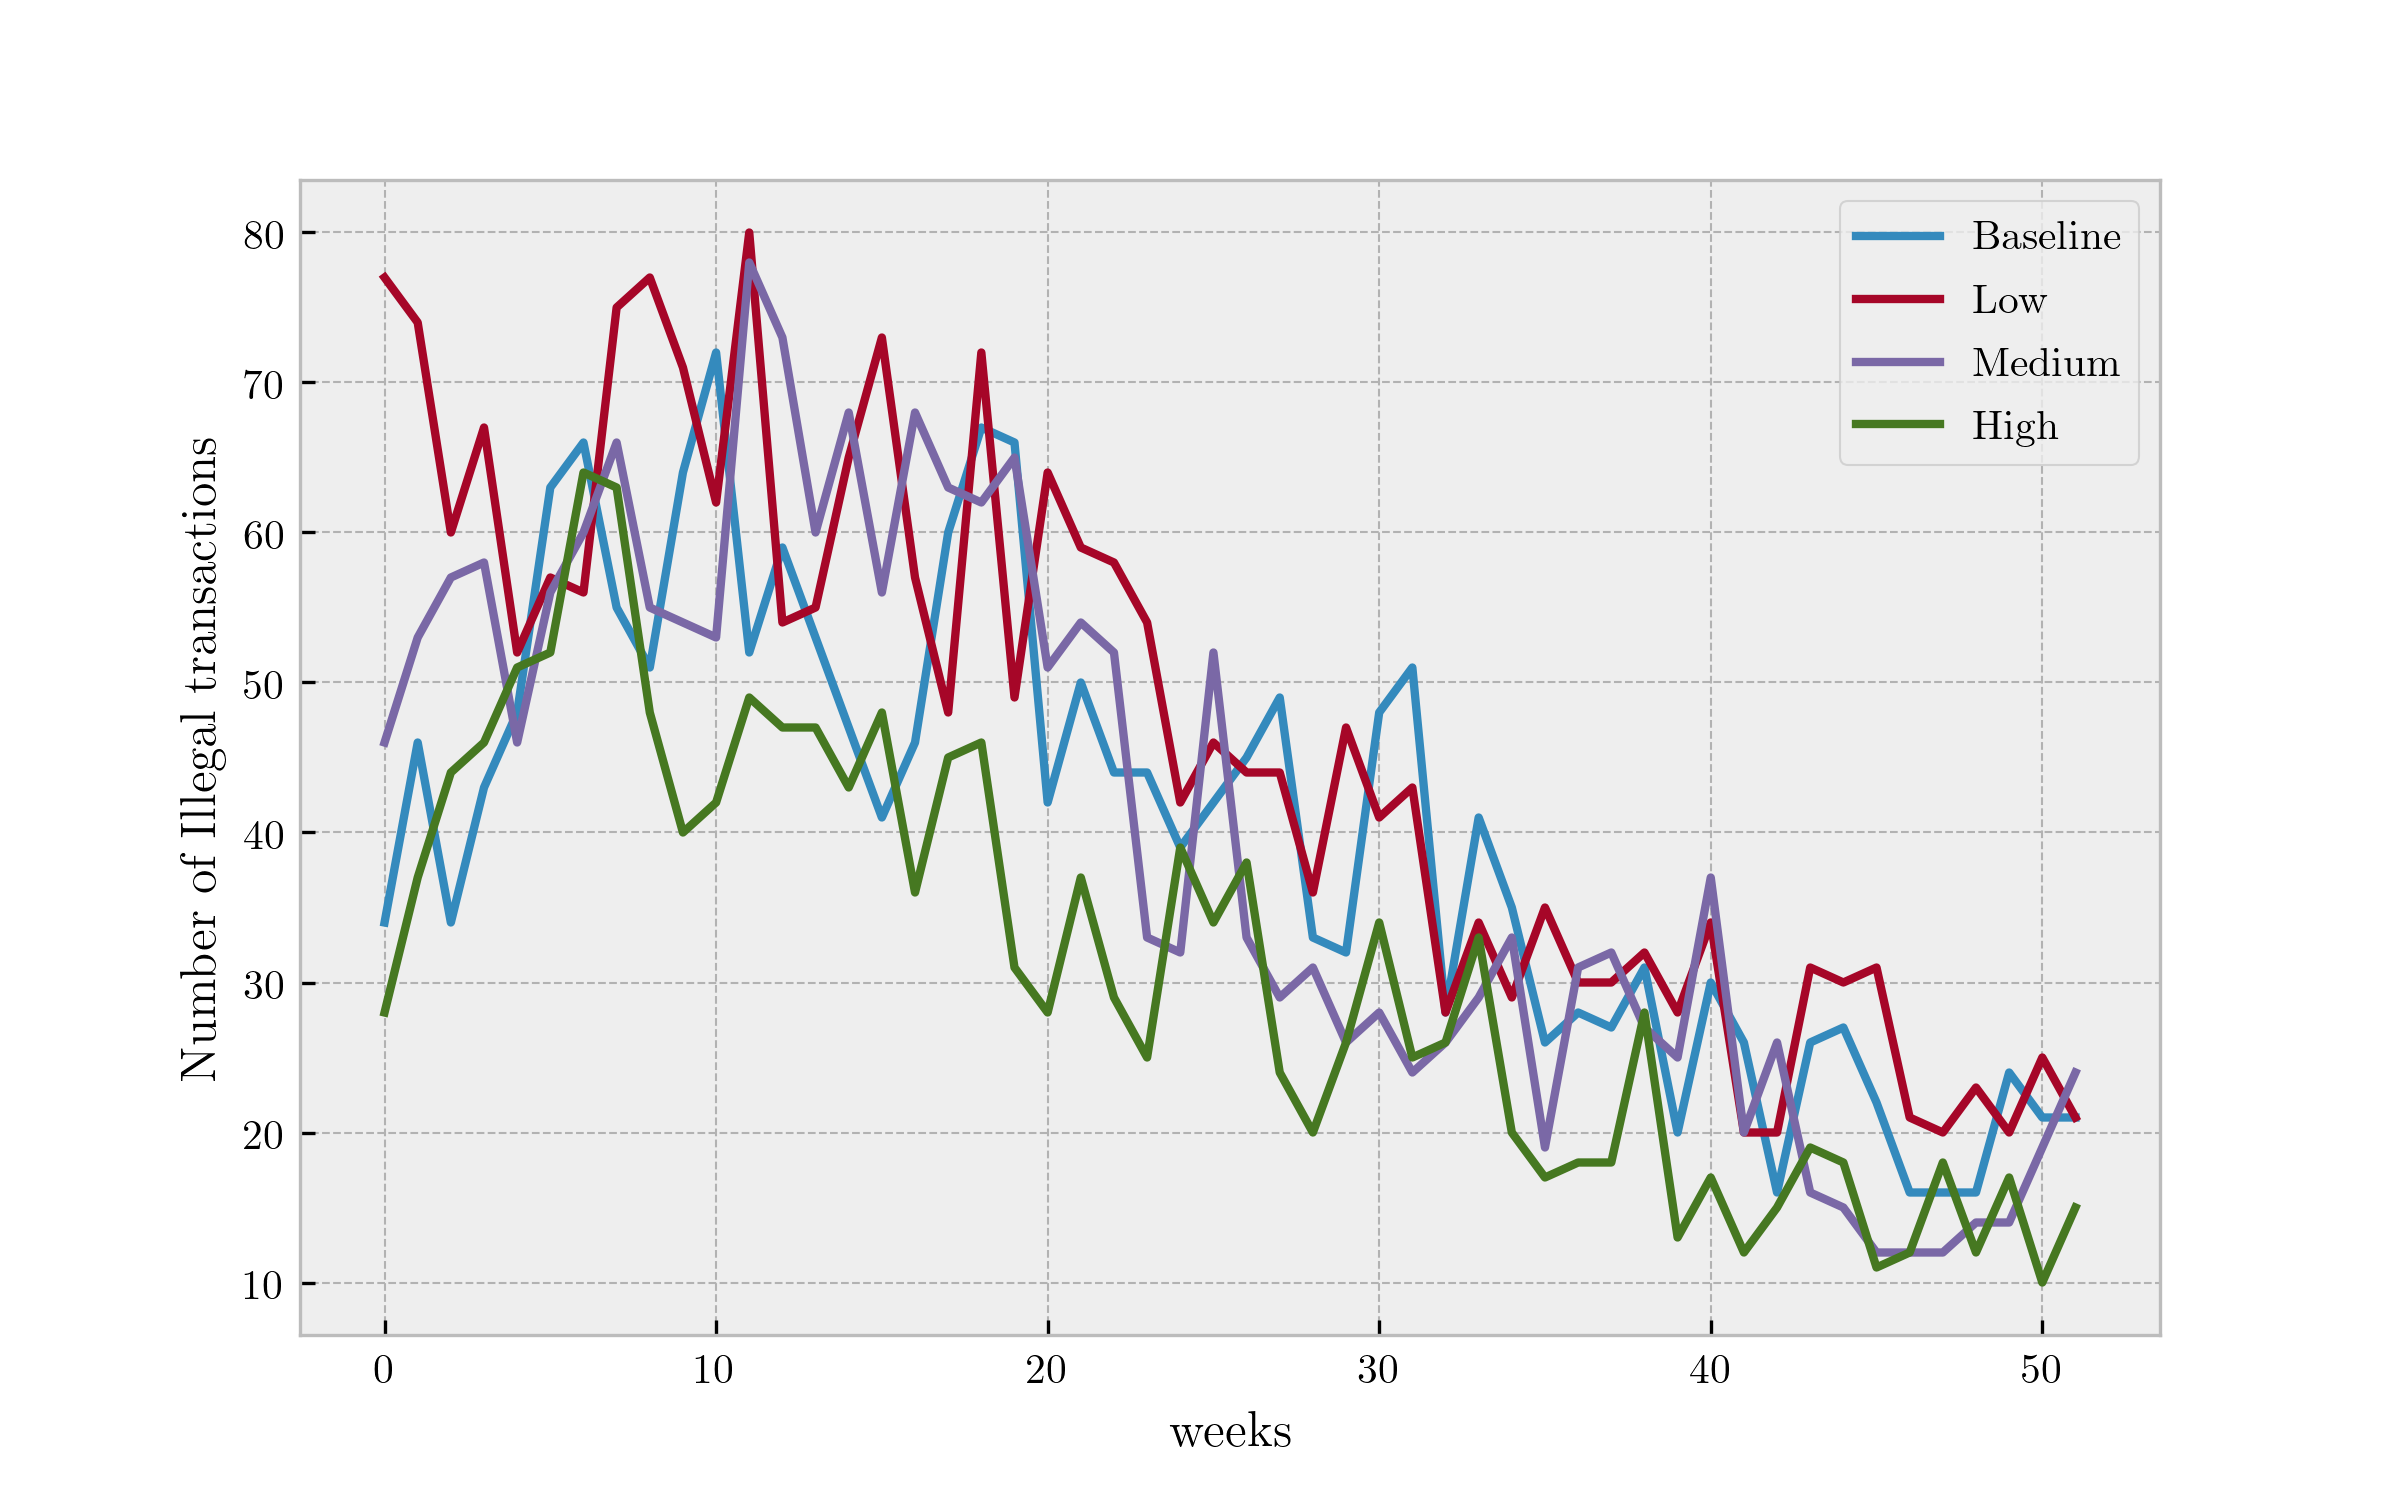
\includegraphics[width=.9\linewidth]{img/f5.png}
\caption{\label{fig:org168b7a5}
Different settings for risk aversion, homophily network}
\end{figure}

\subsection{Different starting proportions of corrupt agents}
\label{sec:orgbe1af86}
The final test we performed on the parameters was to see how different proportions of corrupt agents affect the outcome of the model. We used the number of illegal
transaction per week as our outcome; with 1, 20, 40, 60, 80, and 99\% of corrupt agents. The results in Figure \ref{fig:orgca41e02} reproduce what was found by modifying the risk aversion
distribution. However, in case of the proportion of corrupt agents, the extreme case where 99\% of agents are corrupt maintains a higher number of illegal transactions, regardless of how much time has passed, and also appears to decrease at the same rate.

\begin{figure}[htbp]
\centering
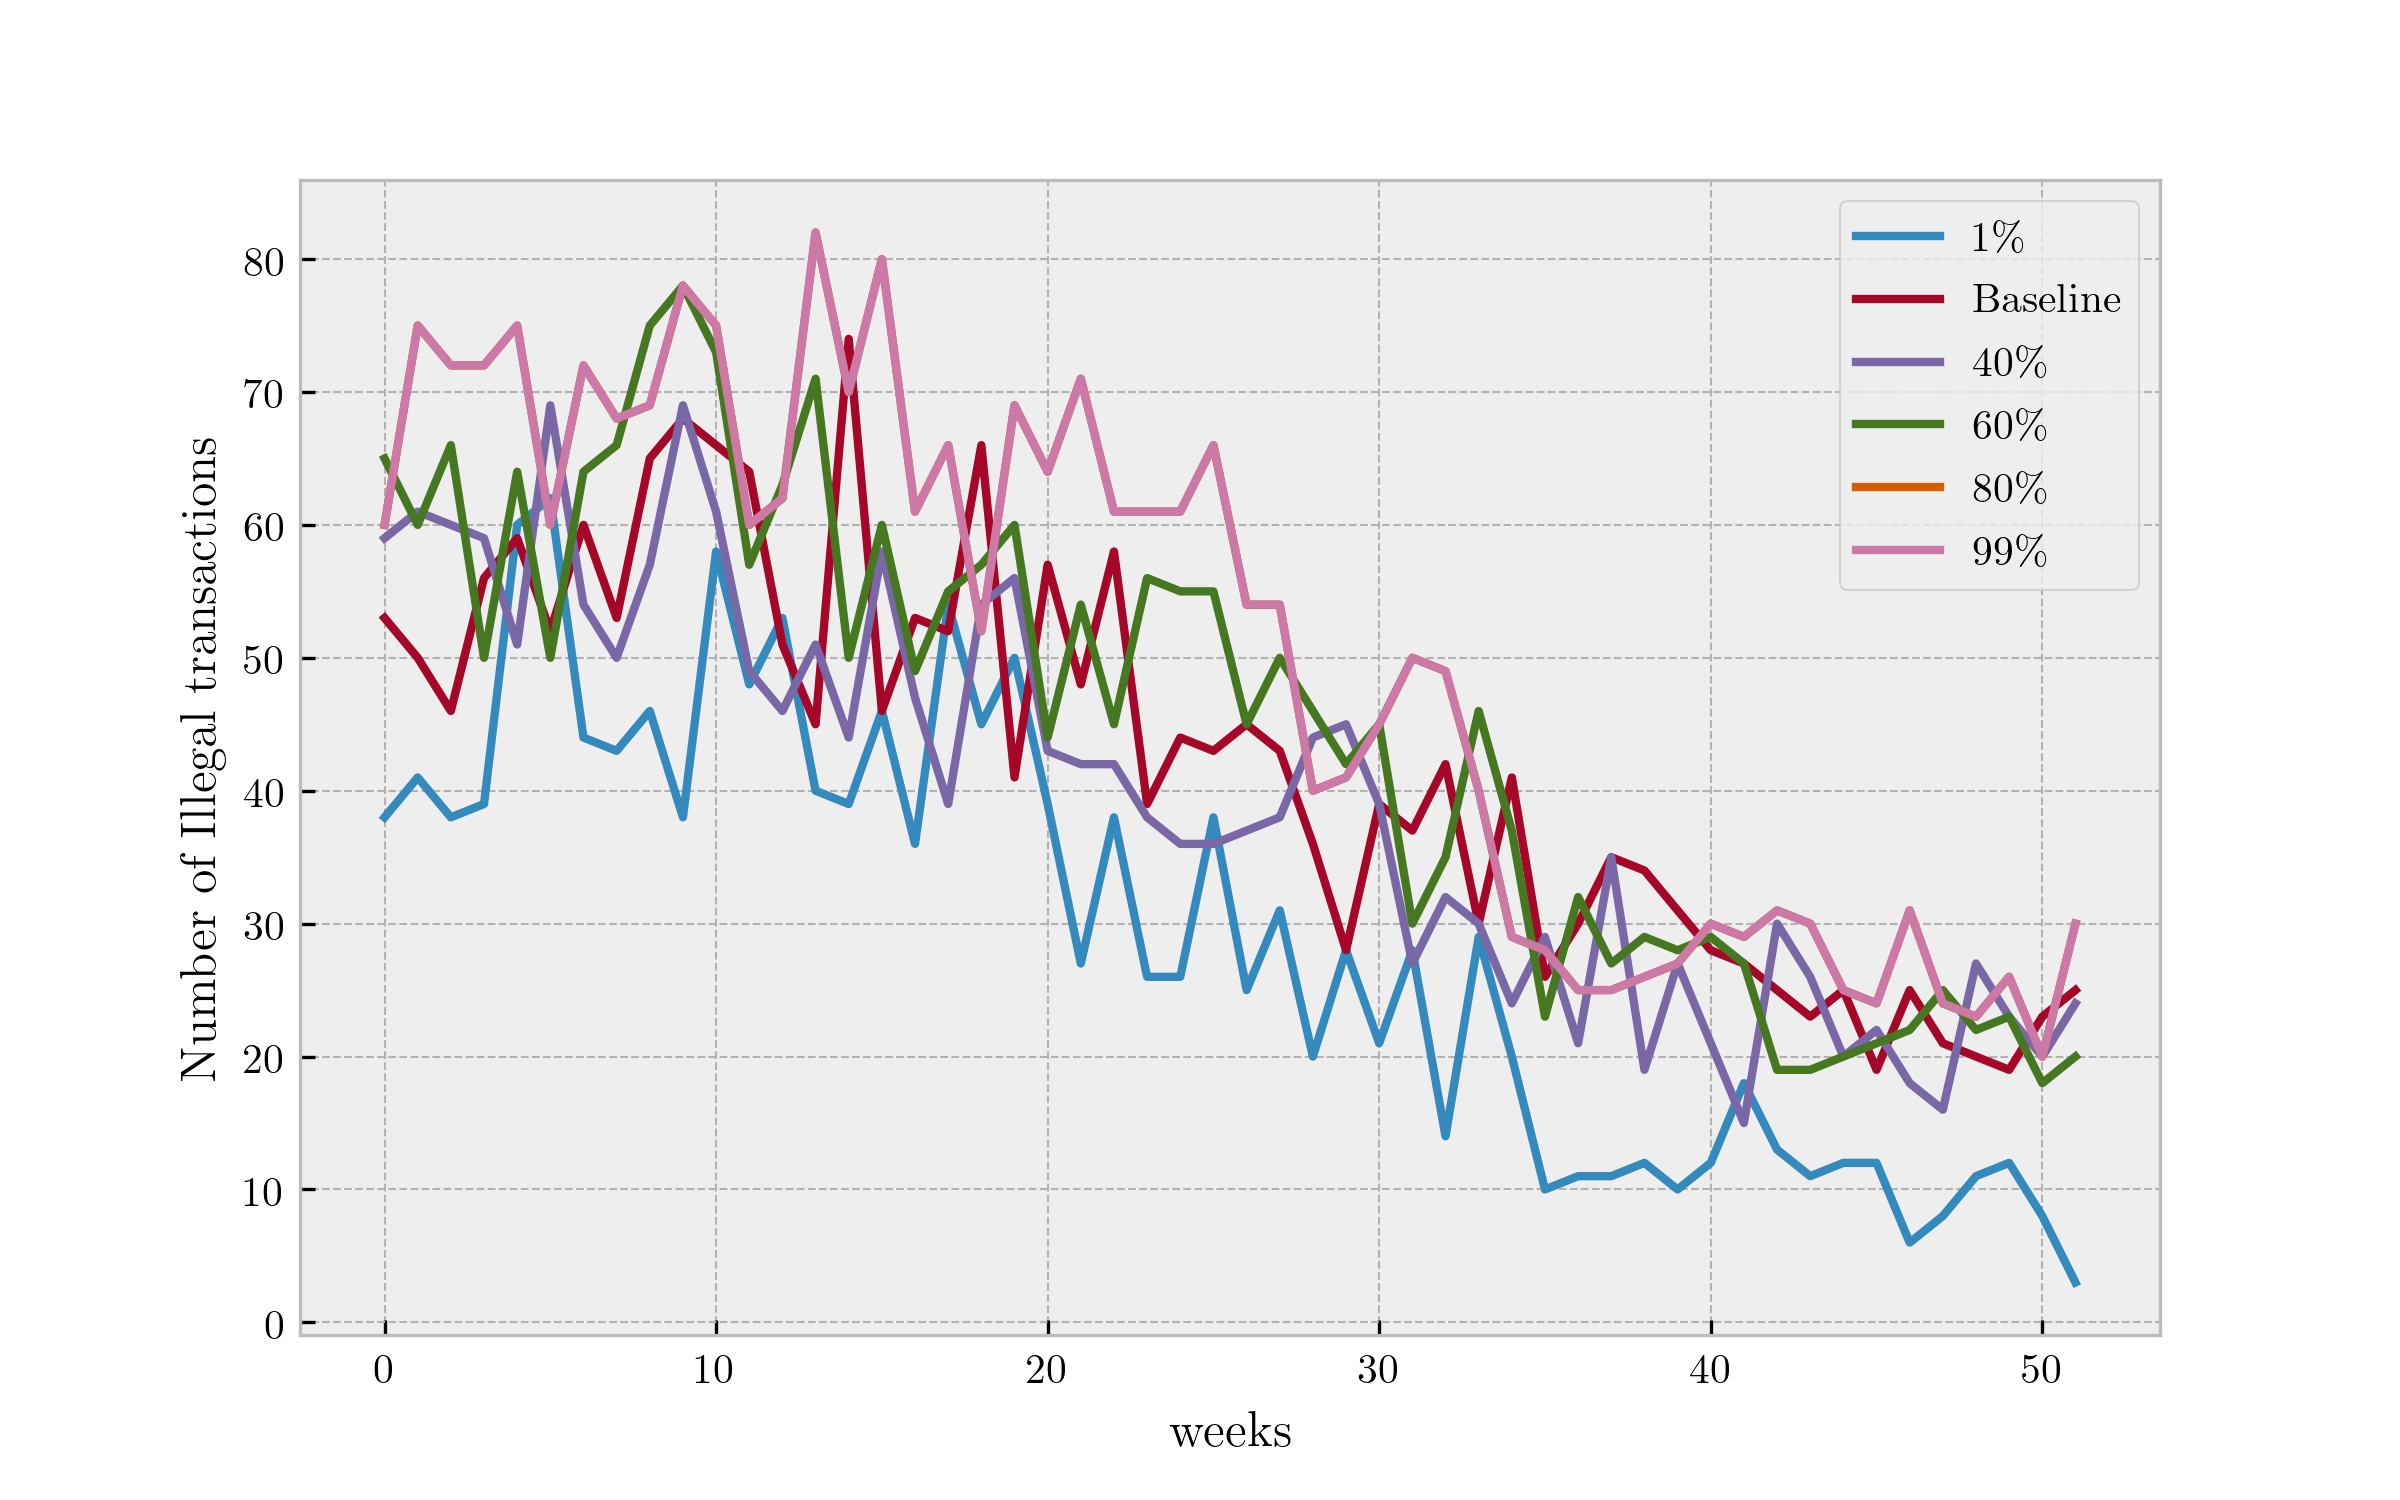
\includegraphics[width=.9\linewidth]{img/f6.png}
\caption{\label{fig:orgca41e02}
Different setting for risk aversion with different percentages of corrupt agents, homophily network.}
\end{figure}

\section{Conclusion}
\label{sec:org5c5327f}
As we mentioned earlier,a closer look at the linkages between the major players in the \emph{Lava Jato} case, allow us to better understand the patterns of corruption in this case, and how individual choices from the bottom-up can have created large scale illegal activities. We learn from the results of our model that small world networks are the ones where the illegal transactions are low and stable. Therefore, what happened in Brazil clearly was not a small world, and it also wasn’t random. This helps show that we have evidence to think that there was a homophily process in the formation of the corruption network. Homophily networks as a more specific topic within this corruption scandal would also be an interesting investigation in future works, particularly with  new data and networks that are revealed as the investigation develops.

This is a theoretical model based on the details we have of the \emph{Lava Jato} investigation thus far, and it does show similar behavior to the known networks that have already been revealed. Despite what we know of the investigation, there is limited data for us to thoroughly validate this model. Our results are robust and conceptually represent the way in which corruption occurs and has an effect on others within a network, but real data could provide more information about the structures of the networks, and the motivations and decision-making processes of the individuals engaged in corruption. However, even with additional data, we would at most have the illegal transactions that occurred, but not the attempted ones- which may be another benefit of simulating these types of behaviors to understand corruption. 

While our results are consistent, further experimentation with empirical data and different model assumptions may produce variations of these results. Gaining a better understanding of the linkages between the major players can also help with targeted corruption detection and prevention. In further works, we can experiment with targeting links and targeting nodes to understand what types of strategies can be effective in cases of large-scale corruption, as well as experimenting with removing nodes from the network, targeting specific types of agents (highest degree, centrality, etc) to understand the influence and relationship. By building an agent-based model to look at the frequencies of agents committing crimes and engaging in corruption, we can explore the different thresholds and understand what types of effects result in higher proportion of agents committing crimes, as well as understanding if some types of social networks are more or less vulnerable to crime detection. 

Overall this model serves as a theoretical representation of corruption within the case of the \emph{Lava Jato} scandal and understanding these networks and effects can help enhance our understanding of individual behaviors with large-scale impacts. Modelling can show clearer patterns and underlying networks, which can lead to better policies that can be implemented to combat corruption in the early stages.

\bibliographystyle{/home/vsvh/bibstyles/asr.bst}
\bibliography{references} 
\end{document}